\chapter{Cloud Computing} 
\label{ch:cloud}
Das erste Kapitel hat deutlich gemacht, welche Anforderungen im Hochschulsport an ein Software System gestellt werden, sowie welchen Dynamiken und Besonderheiten das fachliche Umfeld unterliegt. In diesem Kapitel soll ein Verständnis für unterschiedliche Softwarearchitekturen und Vertriebsmodelle geschaffen werden. Dabei soll vor allem auf das Thema Cloud Computing eingegangen werden, welches an Bedeutung gewinnt und Gegenstand vieler akademischen und wirtschaftlichen Beiträgen in der Fachpresse ist. 
\\

Für den Begriff Cloud Computing finden sich in der Literatur vielfältige Definitionen. Die häufigste Verwendung findet jedoch die Definition des National Institute of Standards and Technology (NIST), dessen Definition sich auch die European Network and Information Security Agency (ENISA) angeschlossen hat, in der Form:

\begin{quote}
	Cloud computing is a model for enabling ubiquitous, convenient, on-demand network access to a shared pool of configurable computing resources (e.g., networks, servers, storage, applications, and services) that can be rapidly provisioned and released with minimal management effort or service provider interaction. This cloud model is composed of five essential characteristics, three service models, and four deployment models.
\end{quote} \cite*[vgl.][S.2]{Mell.2011}\\

Diese Definition des ist auch Grundlage für die Definition des Bundesamt für Sicherheit in der Informationstechnik (BSI) welches den Begriff Cloud Computing folgendermaßen festlegt:
\begin{quote}
	Cloud Computing bezeichnet das dynamisch an den Bedarf angepasste Anbieten, Nutzen und Abrechnen von IT-Dienstleistungen über ein Netz. Angebot und Nutzung dieser Dienstleistungen erfolgen dabei ausschließlich über definierte technische Schnittstellen und Protokolle. Die Spannbreite der im Rahmen von Cloud Computing angebotenen Dienstleistungen umfasst das komplette Spektrum der Informationstechnik und beinhaltet unter anderem Infrastruktur (z. B. Rechenleistung, Speicherplatz), Plattformen und Software.
\end{quote} \cite*[vgl.][]{BundesamtfurSicherheitinderInformationstechnik.}

\section{Merkmale}
\subsubsection{On-demand self-service}\label{selfservice}
\subsubsection{Broad network access}\label{networkaccess}
\subsubsection{Resoruce pooling}\label{resourcepooling}
\subsubsection{Rapid elasticity}\label{rapidelasticity}
\subsubsection{Measured service}\label{measuredservice}
\cite*[vgl.][S.2]{Mell.2011}

\section{Service Modell}\label{serviceModell}
In der Definition von \cite*[S.2]{Mell.2011} sind drei unterschiedliche Service Modelle beschreiben, die sich in der Cloud Community etabliert haben. Diese decken sich mit den Kategorisierungen von \cite[S. 28]{Tharam.2010} und \cite[S. 878]{Jadeja.2012}.

	\begin{figure}[h]
		\centering
		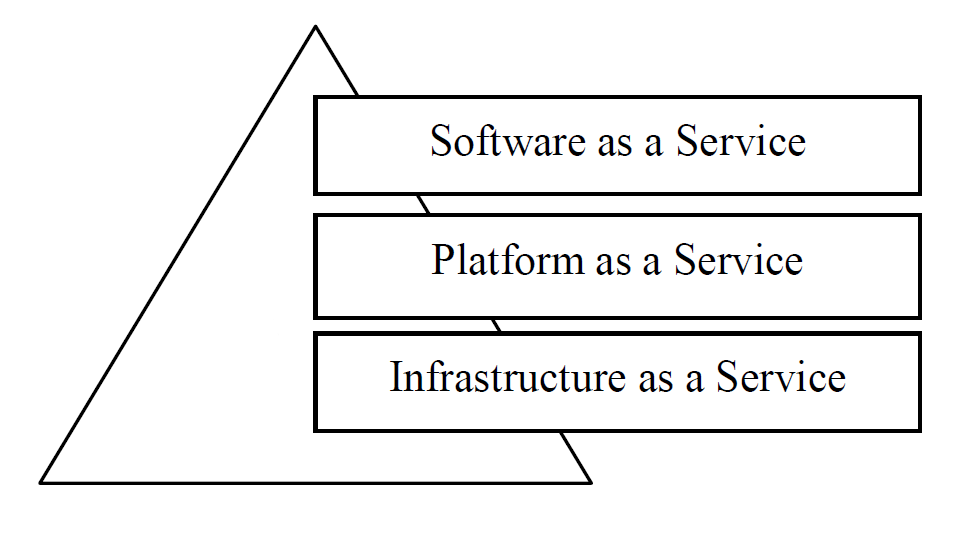
\includegraphics[width=0.5\linewidth]{images/cloud_computing_pyramide}
		\caption{3-Ebenen Modell von Cloud Computing}
		\label{fig:CloudComputingPyramide}
	\end{figure}


\textbf{Software-as-a-Service (SaaS)} stellt eine Anwendung in der Cloud bereit, die von Nutzern verwendet werden kann, ohne eine eigene Installation vornehmen zu müssen. Der Nutzer hat dabei keinen Zugriff auf die Cloud Infrastruktur. Wichtige Merkmale einer SaaS Anwendungen sind Netzwerk basierter Zugriff, Nutzer können limitierte spezifische Konfigurationen vornehmen und sind meistens als Multi-Tenancy-System aufgebaut. Beispiele sind Anwendungen wie SalesForce.com, Google Mail, Google Docs, Office 365, Quicken Online, etc.
\\

\textbf{Platform as a Service (PaaS)} bezeichnet Software und Entwicklungstools, die der Nutzer verwenden kann, um eigene Anwendungen zu entwickeln und zu veröffentlichen. Der Nutzer hat dabei keinen Zugriff auf die darunter liegende Cloud Infrastruktur, kann jedoch im Vergleich zu SaaS die eigene Anwendung frei konfigurieren. Beispiele für PaaS Services ist Google AppEngine.
\\

\textbf{Infrastructure as a Service (IaaS)} ist die unterste Ebene der Cloud Computing Pyramide. Dem Nutzer wird virtualisiert Hardware wie Datenspeicher, Virtuelle Maschinen, Netzwerke, etc. zur Verfügung gestellt, die frei verwendet werden können. IaaS Services werden gewöhnlich auf pay-per-use Basis bezahlt. Amazon EC2, VMWare und Windows Azure sind nur einige Beispiele.
\\

In einigen Fällen werden diese drei Ebenen noch um zusätzliche Service Formen ergänzt. So verwendet \cite[S. 28]{Tharam.2010} noch die Einteilung in storage as a Service (DaaS) während \cite[S. 123]{Mahmood.2011} von other Provision as Service spricht und darunter Formen wie Storage as a Service, Database as a Service, Security as a Service, Communication as a Service, etc gruppiert. All diese Services können jedoch auch als spezialisierte IaaS Services angesehen werden und sollen daher in dieser Arbeit keine weitere Betrachtung erfahren.


\section{Bereitstellung Modell}\label{bereitstellung}
Ein weiterer zentraler Punkt in der Definition von Cloud Computing ist das Bereitstellungsmodell, das primär die Art beschreibt, wer Zugriff auf die Daten und Anwendungen hat.

	\begin{figure}[h]
		\centering
		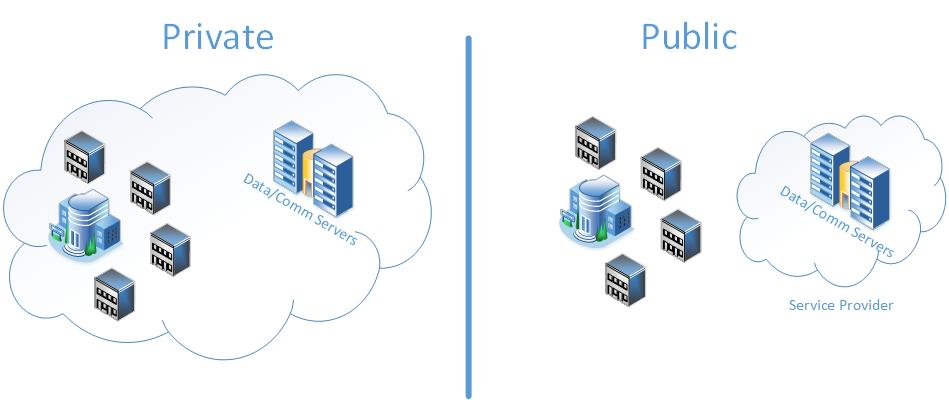
\includegraphics[width=0.9\linewidth]{images/private_public_cloud}
		\caption{Public und Private Cloud Architektur}
		\label{fig:PublicPrivateCloud}
	\end{figure}

\subsection{Private Cloud}
Als Private Cloud wird das Szenario bezeichnet, wenn die Infrastruktur nur von einem Kunden genutzt wird. Im Normalfall ist sie im Organisationseigenen Rechenzentrum beheimatet. Sicherheit, Datenschutz, Wartung sind so einfacher durch eigenes Personal oder externe Dienstleister zu organisieren und zu überwachen. Die Private Cloud lässt sich daher mit einer erweiterten Art des Intranets vergleichen. \cite[S. 879]{Jadeja.2012} \\
\cite{Tharam.2010} nennen fünf Gründe, die für eine Private Cloud sprechen können:
\begin{enumerate}
\item Maximieren und optimieren bestehender, eigenen Ressourcen
\item Sicherheitsbedenken und Datenschutz
\item Datentransferraten
\item Vollständige Kontrolle über kritische Aktivitäten
\item Forschungs- und Ausbildungszwecke
\end{enumerate}

\subsection{Public Cloud}
Dieses Modell ist derzeit in der Öffentlichkeit am besten bekannt. Nutzer können die Cloud über ein Web-Interface ansteuern und bezahlen für die Dauer der genutzten Services. Im Vergleich zu anderen Modellen ist die Public Cloud weniger sicher, da sie leichter zugänglich für bösartige Angriffe ist. Bekannte Public Cloud Anbieter sind Amazon EC2, S3, Google AppEngine, Force.com und Microsoft Azure. \\
(vgl. \cite{Jadeja.2012} und \cite{Tharam.2010})
	
\subsection{Hybrid Cloud}
Bei der Hybrid Cloud handelt es sich um eine Kombination aus zwei oder mehr Cloud Arten, die für sich selbst existieren, aber miteinander verbunden sind. Dadurch lassen sich eine Private und Public Cloud einfach kombinieren und Sicherheitsanforderungen kann gerecht geworden werden. Dies ist in erster Linie möglich wenn Datenschutz und Sicherheitskritische Anwendungsteile in die Private Cloud verlagert werden, weniger wichtige aber hoch nachgefragte Teile in die Public Cloud gestellt werden.\\
Hybrid Clouds sind die Treiber zur Notwendigkeit einer Standardisierung und Cloud Interoperabilität damit die Clouds miteinander kommunizieren können.

	\begin{figure}[h]
		\centering
		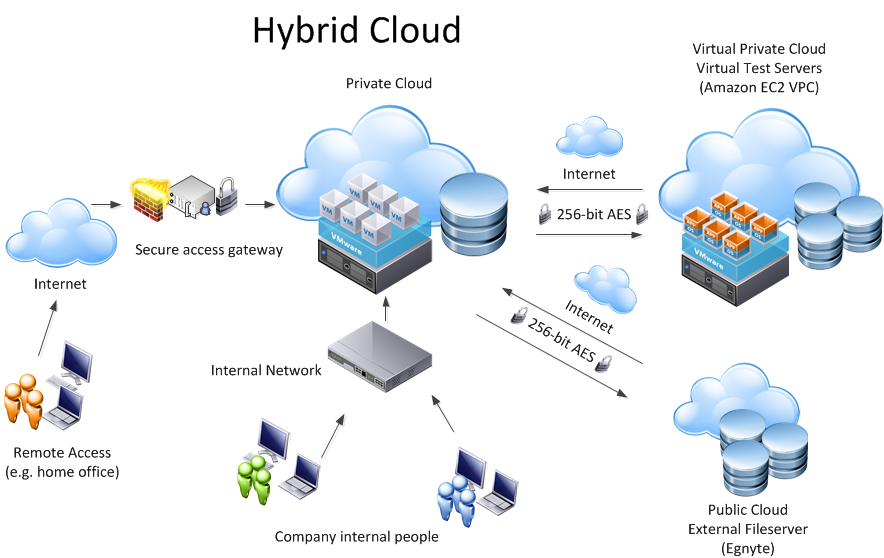
\includegraphics[width=0.9\linewidth]{images/hybrid-cloud-architektur}
		\caption{Hybrid Cloud Architektur}
		\label{fig:HybridCloud}
	\end{figure}


Community Cloud\\

\section{Pro \& Contra}
Nachdem der Begriff Cloud Computing, sowie die beinhalteten Service und Bereitstellungsmodelle erläutert wurden stellt sich die Frage nach den Vor- und Nachteilen dieses neuen Modelles. Wie bei den meisten neuen Entwicklungen und Technologien ist die Entstehung getrieben aus den Unzulänglichkeiten bestehender Ansätze und so können die Merkmale, die diese Neuentwicklung definieren in vielen Fällen auch als Vorteile angesehen werden. Nachdem einige Gründe der Notwendigkeit bereits in Abschnitt~\ref{herausforderungen} erläutert wurden sollen hier die Vor- und Nachteile jedoch noch einmal explizit zusammen gefasst werden. Der Fokus liegt hierbei vor allem auf den Services IaaS und PaaS, die etwas anders betrachtet werden können als SaaS. Auch wenn viele der Vor- und Nachteile auch für SaaS Modelle gelten, werden diese im Abschnitt~\ref{SaaS} noch einmal explizit betrachtet. Verglichen werden dabei Cloud Anbieter mit dem traditionellen Rechenzentrum.

\subsection{Vorteile}

\subsubsection{Einfachheit}\label{einfachheit}
Cloud Angebote leben von ihrer einfachen Einrichtung. Speziell als Anwender bzw. Kunde genügt in den meisten Fällen ein Webbrowser, um sich auf der entsprechenden Oberfläche die benötigten Ressourcen anzufordern und automatisiert bereit gestellt zu bekommen. Es handelt sich hier um eine Art Outsourcing, sodass die Fachkenntnis auf Hardware- und Softwareebene nicht mehr in der Tiefe notwendig ist, wie sie bei einem eigenen Betrieb vorhanden sein muss, um ein gleichen Qualitätslevel zu erreichen.
\subsubsection{Kostenersparnis}\label{kostenersparnis}
Der Faktor Kostenersparnis gilt als einer der größten Vorteile, wobei die Berechnung der Kostenersparnisse für IT nicht all zu trivial ist, da sich je nach Modell diese ggf. erst nach Jahren rentieren. Die Kosten mit eigener Verantwortung für die Bereitstellung und Unterhaltung ergeben sich primär aus den Beschaffungskosten für Hardware, Software und zusätzlich anteilig an den Personal- oder Dienstleisterkosten für Wartung und Instandhaltung. Mit einbezogen werden muss dabei zusätzlich, dass ggf. Neuanschaffungen und Erweiterungen über die Jahre notwendig sein werden.\\
 Die Preismodelle von Cloud Anbietern wie Amazon Web Services (AWS), Microsoft Azure (Azure) oder Google AppEngine (AppEngine) unterscheiden sich dabei sehr von den traditionellen Abrechnungsmodellen. Auch wenn nicht jeder Anbieter alle Modelle unterstützt, so haben sich doch Abrechnungen nach Datenvolumen (wie viel Speicherplatz wird bereit gestellt), Computer Ressourcen (wie viel Arbeitsspeicher und CPU wird beansprucht), Datentransfervolumen (wie viel Datenvolumen wird über das Netzwerk transferiert) und einige andere in der Praxis etabliert. Der große Unterschied liegt jedoch in der Kombination mit dem Skalierbarkeitsfaktor. So wird im Gegensatz zum traditionellen Rechenzentrum nur das bezahlt, was wirklich benutzt wird und überschüssige Ressourcen können bei Bedarf einfach zurück gegeben werden. In der Literatur gibt es für diese Abrechnungsform jedoch bisher keinen einheitlichen Begriff und wird unterschiedlich als utility-style pricing, pay-as-you-go oder pay-per-use bezeichnet. (vgl. \citeauthor*[S. 879]{Jadeja.2012}; \citeauthor*[S. 313]{Achimugu.2012}) \\
 Wie groß die Kostenersparnisse im Detail sein können ist sehr abhängig von den aktuellen Preisen, der Anwendungsarchitektur und der kalkulierten Laufzeit. In den letzten Jahren hat sich bei den Anbietern Amazon, Microsoft und Google ein richtiger Preiskrieg entwickelt, der zu stetig fallenden Preisen geführt hat und so die Kostenersparnisse weiter vergrößert hat. 

\subsubsection{Skalierbarkeit und Flexibilität}\label{skalierbarkeit}
Elastizität und Skalierbarkeit ist ein weiter Hauptvorteil von Cloud Umgebungen. Datenspeicher und Computing Power steht in fast unbegrenzter Menge zur Verfügung und können mit wenigen Handgriffen vom User über einen Self-Service dazu provisioniert werden. So wie die Erweiterung der Ressourcen einfach möglich ist, so lassen sich diese auch wieder zurück geben wenn sie nicht mehr benötigt werden. Zusammen mit einer pay-per-use Abrechnung führt dies dazu, dass zusätzlich Ressourcen ggf. nur für bestimmte Zeiträume in Anspruch genommen werden müssen. \\
In traditionellen Rechenzentren ist das kurzzeitige hinzu schalten neuer Ressourcen und das anschließende Zurückgeben schwieriger. Werden neue Ressourcen benötigt, so stehen diese nur begrenzt zur Verfügung. Durch unterschiedliche Virtualisierung Umgebungen hat dies zwar auch zu mehr Flexibilität geführt, jedoch sind die Möglichkeiten begrenzt. Auch die Zeit, die bis zur Bereitstellung neuer Ressourcen benötigt wird ist im Normalfall deutlich länger, da der Prozess weniger automatisiert abläuft. Je mehr diese Automatisierung integriert ist, desto eher bewegt sich die Lösung im Bereich der Private Cloud.

\subsubsection{Zukunfts- und Ausfallsicherheit}\label{zukunftssicherheit}
Ausfälle von Hardwarekomponenten ist in der Informationstechnologie ein Fakt der sich nicht vermeiden lässt und unterscheidet sich nicht in Cloud und eigenen Rechenzentren. Gerade in den großen Rechenzentren mit tausenden von Servern ist die Wahrscheinlichkeit für ein Auftreten eines solchen Ausfalles deutlich höher. Mit Redundanz und das Vermeiden von single point of failures wird versucht den Hardware Ausfall für den Endkunden unsichtbar zu machen und den Betrieb ungestört aufrecht erhalten zu können. \\
Durch die reine Anzahl von Hardware und spezialisiertem Personal sind die Cloud Anbieter in ihren Rechenzentren hier deutlich im Vorteil einen störungsfreien Betrieb zu garantieren. Zudem ist durch den Austausch kaputter oder veralteter Hardware eine sukzessive Erneuerung der Hardware ohne weiter Kosten für den Endkunden gegeben.

\subsubsection{Nachhaltigkeit}\label{nachhaltigkeit}
Green IT, der umweltschonende Betrieb und Herstellung von Informationstechnologie, ist in den letzten Jahren von immer größerer Bedeutung geworden. Cloud Computing kann in diesem Bereich einiges beitragen, da Energiekonzepte einfacher optimiert und Ressourcen besser genutzt werden können. \cite*{Siegele.2008} geht von einer durchschnittlichen Auslastung von Hardware Ressourcen mit 5\%-20\% in traditionellen Rechenzentren aus. Was auf den ersten Blick sehr wenig erscheint begründet sich darin, das in Lastspitzen die benötigten Ressourcen um ein 2 bis 10-faches steigen. Um diesen Anforderungen gerecht zu werden, wird in vielen Fällen eine Provisionierung auf Basis des maximalen Workloads vorgenommen und führt zur Ressourcen- und Energieverschwendung in weniger aktiven Zeiten.\\
Durch das einfache hinzufügen von Ressourcen und die interne Ressourcen Verwaltung modernen Cloud Rechenzentren kann dies die Auslastung der einzelnen Systeme auch bei geringer oder moderater Belastung verbessern und so seinerseits zur Umweltschonung beitragen. 

\subsubsection{Beispiel für Vorteile}
Diese Vorteile lassen sich an einem kleinen Beispiel im Hochschulsport mit fiktiven Zahlen verdeutlichen. Wie bereits in Abschnitt~\ref{hspAnforderungen} beschrieben kommt es zu einem enormen zusätzlichen Performance Bedarf für das Buchungssystem zum Buchungsstart. Als Lastspitze wird ein fiktiver Bedarf von 100 Servern zu Grunde gelegt. Diese Lastspitzen treten etwa 10 mal im Jahr auf und halten für 24 Stunden an. Den Rest der Zeit besteht ein Workload für etwa 20 Server. Daraus ergibt sich über das Jahr ein durchschnittlicher Bedarf von 532,6 Serverstunden je Tag. Für eine Veranschaulichung des Kostenfaktors wird eine Serverstunde mit 50 Cent veranschlagt.
\\
\\
Serverstunden je Tag:    $\displaystyle \frac{((355 * 20) + (10 * 100)) * 24}{365}\; =\; \textbf{532,6}	 $\\
\\
Kosten je Tag:           $\displaystyle \frac{532,6 * 50}{100}\; =\; \textbf{266,3€} $\\
\\
Um den Kunden auch in den Lastspitzen die benötigte Performance zusichern zu können, so müsste in einer traditionellem Rechenzentrum die Bemessung des Bedarfs am Peak Load erfolgen und somit für 100 Server. Gemessen am durchschnittlichen Bedarf über das Jahr stellt dies jedoch eine deutliche Überprovisionierung da (\ref{fig:overprovisioning}).
	\begin{figure}[h]
		\centering
		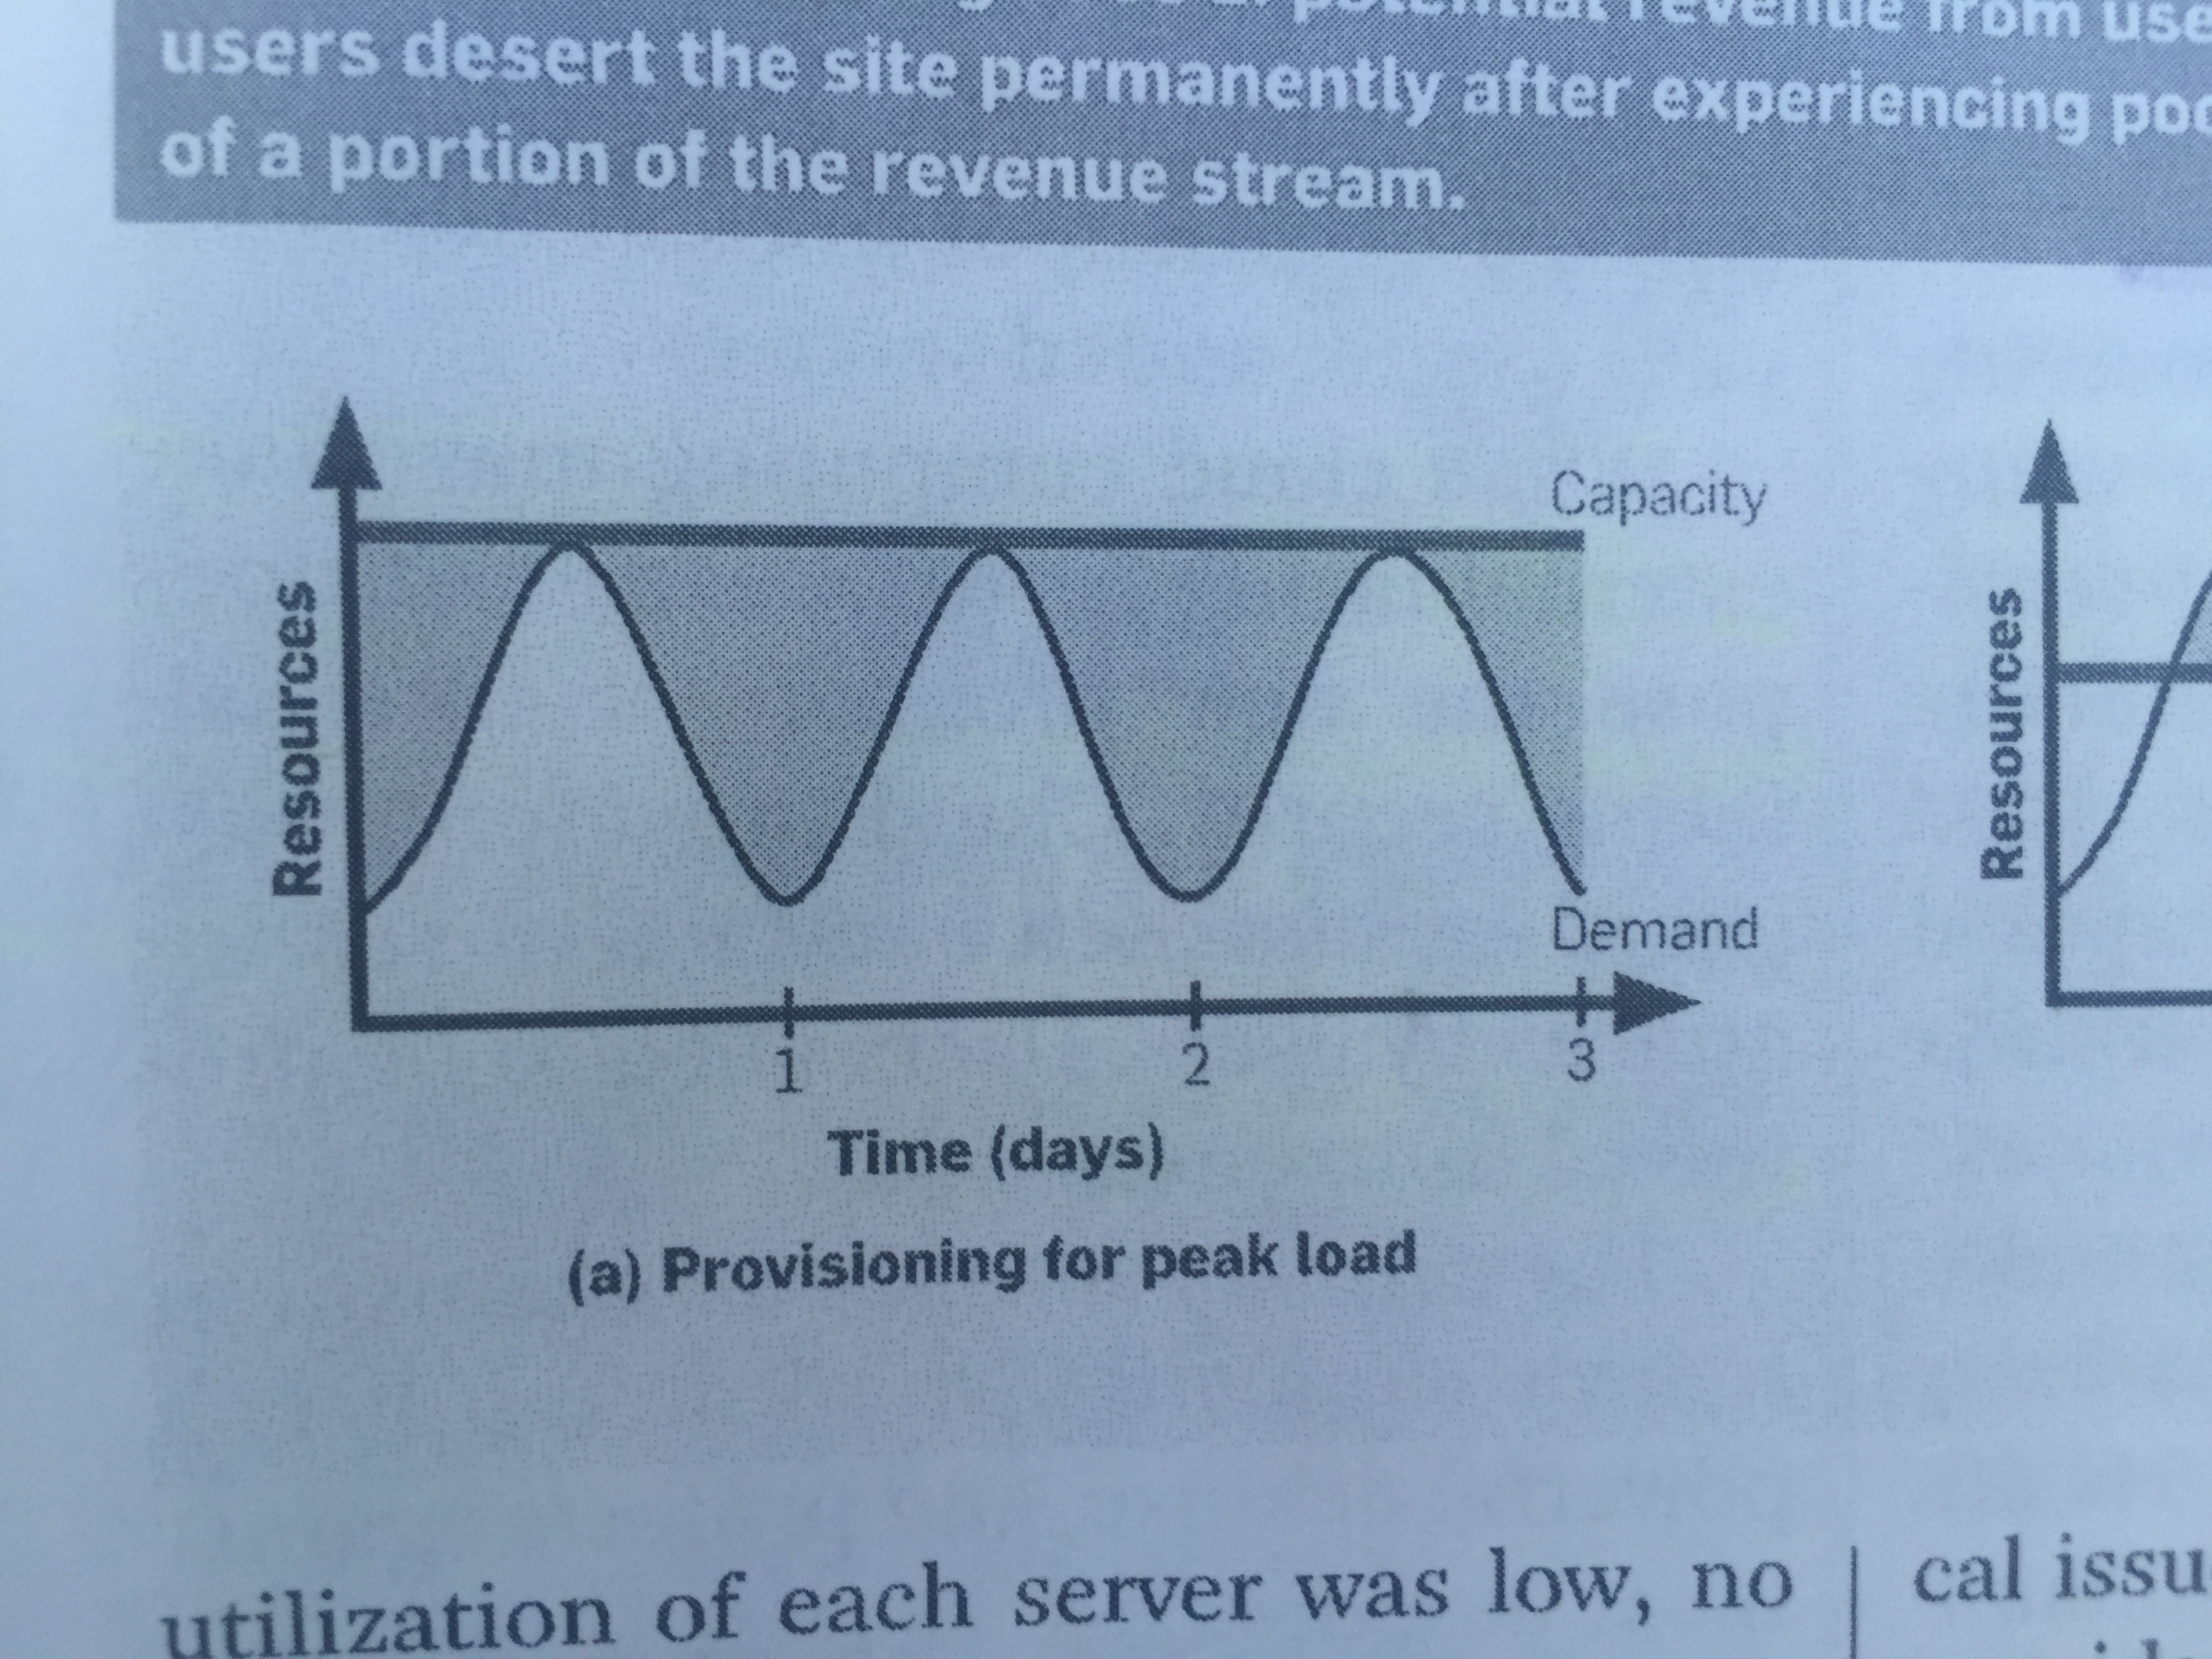
\includegraphics[width=0.7\linewidth]{images/overprovisioning}
		\caption{Provisionierung anhand von Lastspitzen}
		\label{fig:overprovisioning}
	\end{figure}
\\ 
\\
Serverstunden je Tag:    $\displaystyle 100 * 24 \; =\; \textbf{2400} $\\
\\
Kosten je Tag:           $\displaystyle \frac{2400 * 50}{100}\; =\; \textbf{1200€} $\\
\\
Dies entspricht einem erhöhten Preis um Faktor 4,5.
\\
Ein alternativer Ansatz wäre eine moderatere Bemessung des Bedarfes mit z.B. 50 Servern und somit einer Unterprovisionierung möglich. Dies würde dazu führen, das die Lastspitzen jedoch nicht mehr entsprechend versorgt werden könnten und es zu Einschränkungen und sogar Ausfällen des System in diesen Zeiten kommen könnte (\ref{fig:underprovisioning}). 
	\begin{figure}[h]
		\centering
		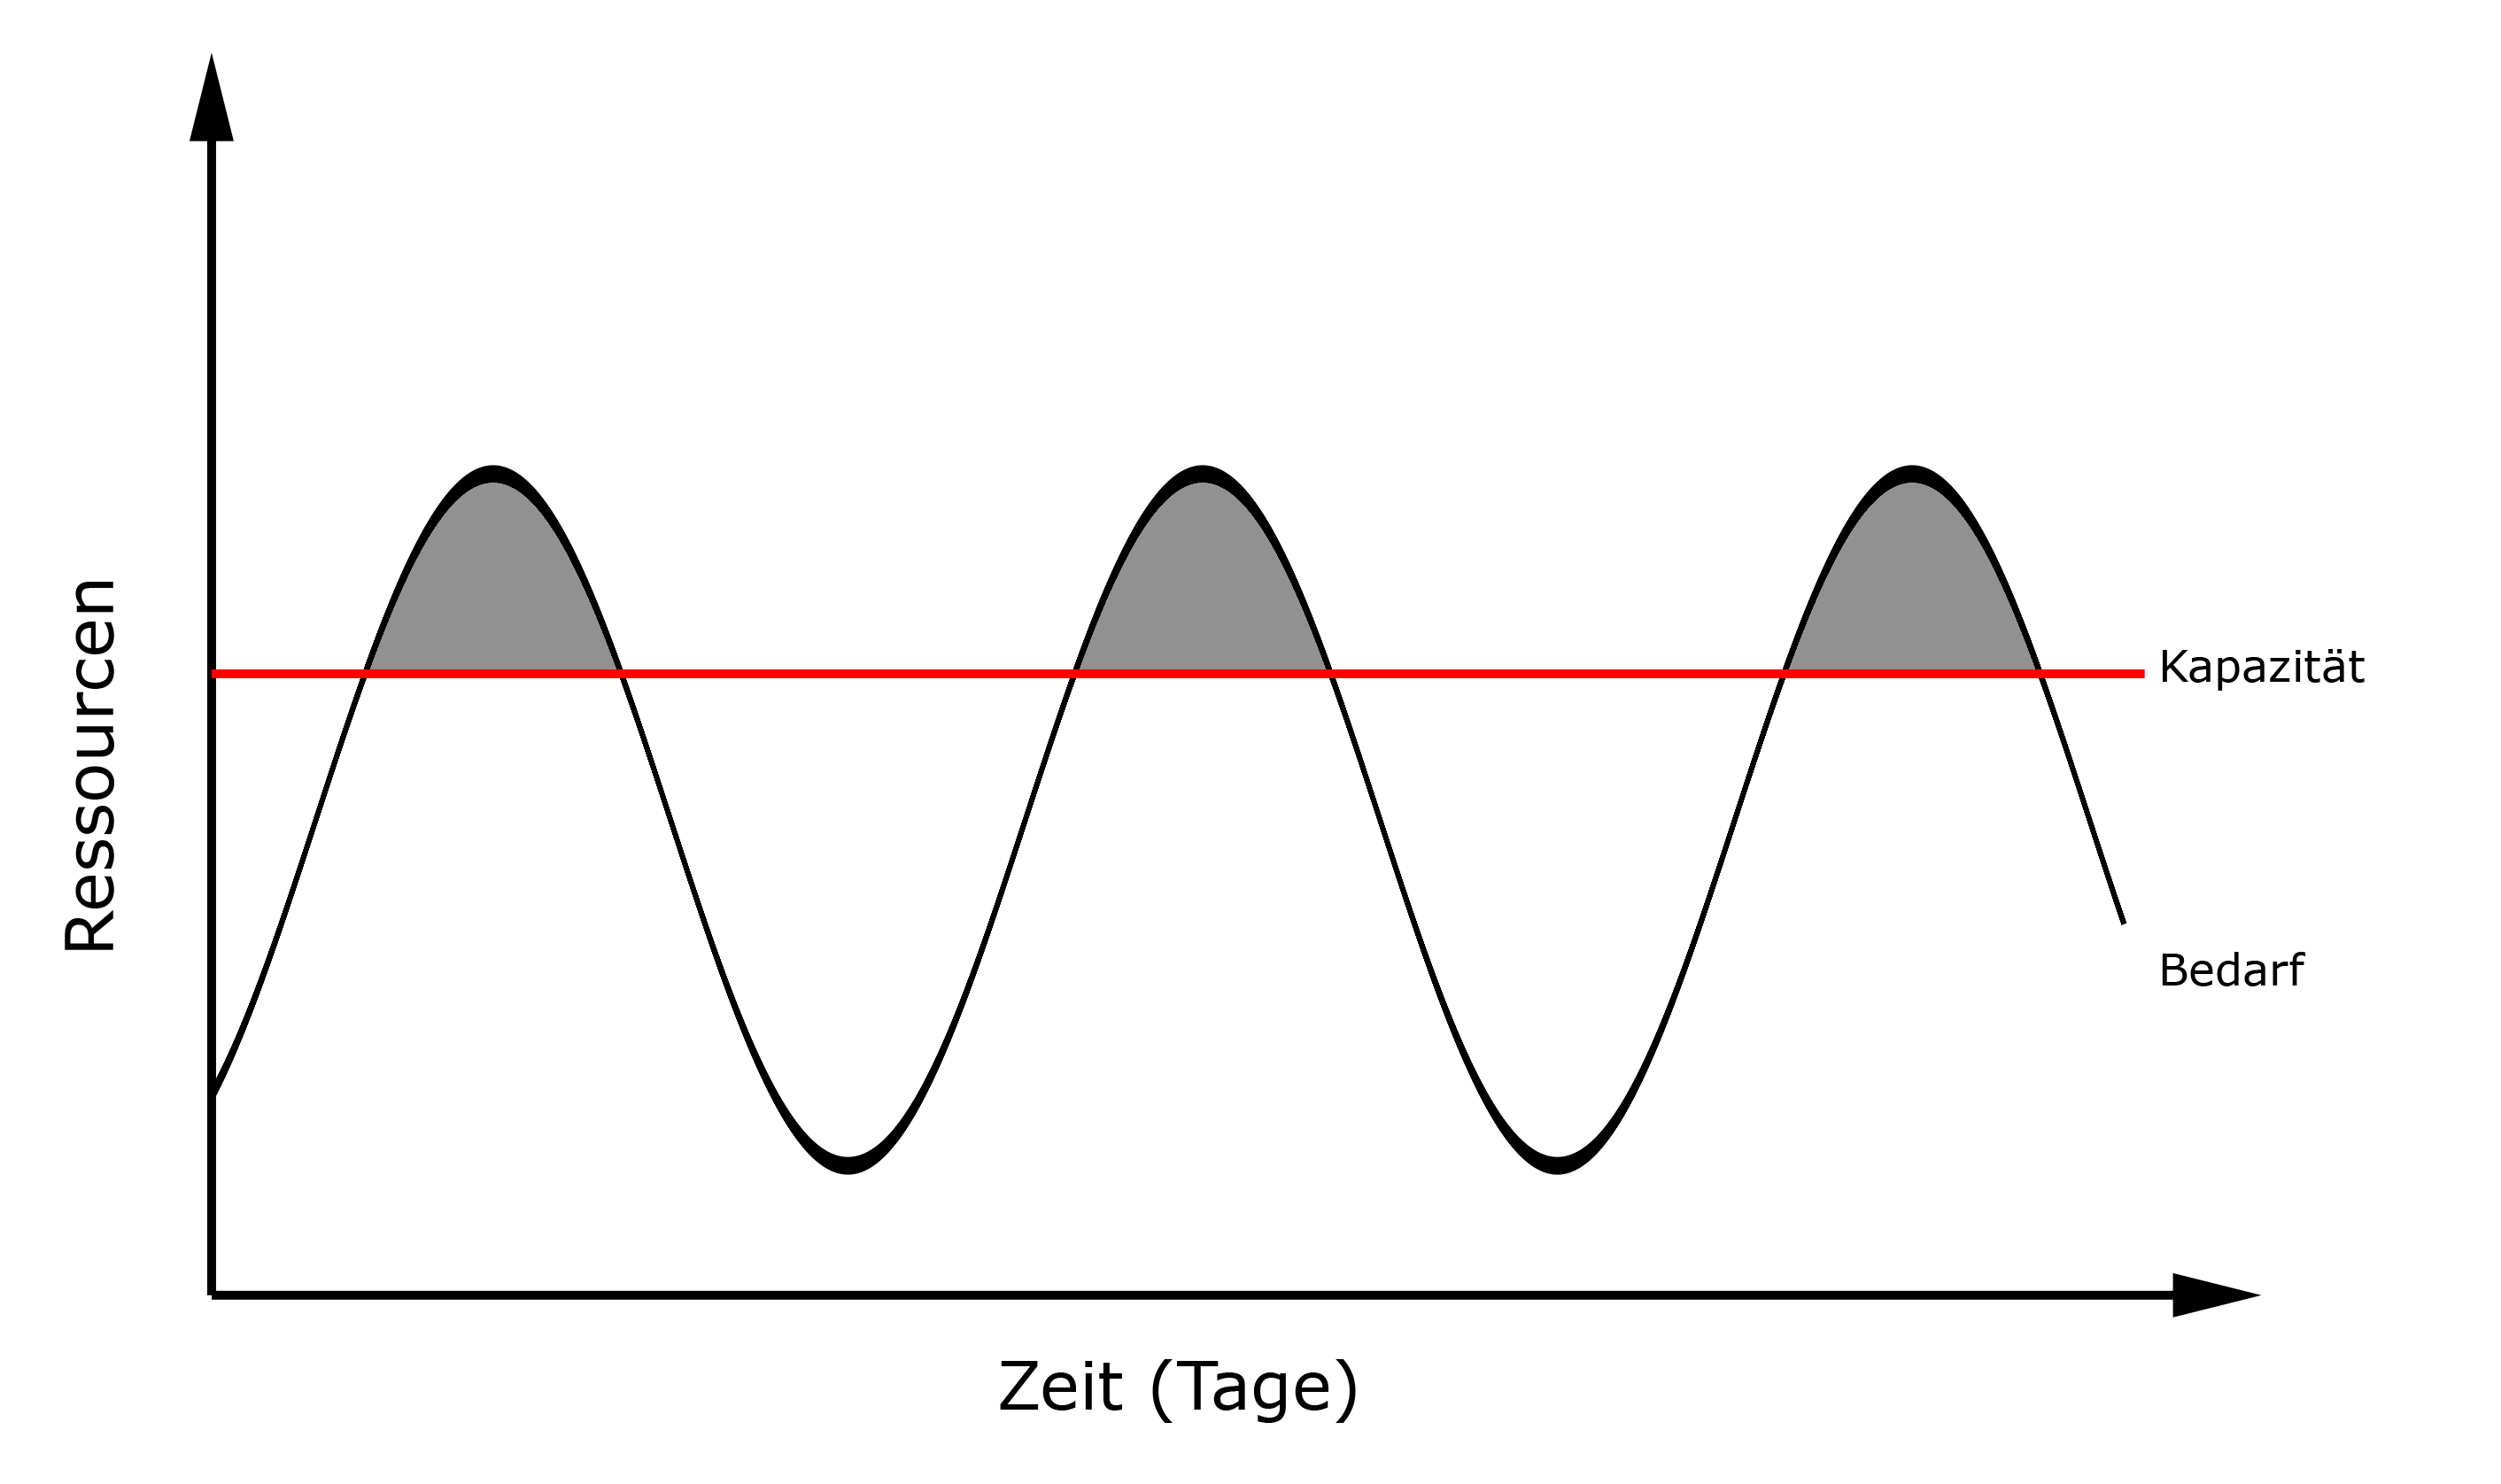
\includegraphics[width=0.7\linewidth]{images/underprovisioning}
		\caption{Unterprovisionierung}
		\label{fig:underprovisioning}
	\end{figure}
Mit diesem Ansatz ließen sich deutliche Einsparungen erzielen, jedoch muss einkalkuliert werden, dass es zu deutlichen Einnahmeeinbußen kommen könnte, da nicht allen Kunden eine Buchung möglich wäre oder sich Kunden sogar vollständig vom diesem Dienst entfernen.
\\
\\
Serverstunden je Tag:    $\displaystyle 50 * 24 \; =\; \textbf{1200}	 $\\
\\
Kosten je Tag:           $\displaystyle \frac{1200 * 50}{100}\; =\; \textbf{600€} $\\
\\
Dieses auf fiktiven Zahlen basierende Beispiel ist in der realen Welt häufig anzutreffen und es müssen mit dem traditionellen Modell Kompromisse eingegangen werden, die unterschiedlich stark ausfallen können. Kosten-Nutzen-Optimierungen sind immer notwendig, bekommen mit dem Cloud Computing aber neue Möglichkeiten. Eine Umsetzung im Cloud Umfeld könnte wie folgt aussehen. Um einen reibungslosen Betrieb in den Phasen mit weniger Aktivität zu gewährleisten und einen gewissen Puffer zu integrieren, werden für das Jahr 25 Server provisioniert. Für die Anmelde Zeiträume werden jeweils für 48 Stunden weiter 75 Server dazu provisioniert. Daraus ergäbe sich folgende Rechnung:
\\
\\
Serverstunden je Tag:    $\displaystyle \frac{((355 * 25) + (20 * 100)) * 24}{365}\; =\; \textbf{715,07}	 $\\
\\
Kosten je Tag:           $\displaystyle \frac{715,07 * 50}{100}\; =\; \textbf{357,53€} $\\
\\
Dies entspräche dem 1,34-fachem des durchschnittlichen Bedarfes und ist in erster Linie dem Puffer geschuldet. Im Vergleich zur Überprovisionierung betragen die Kosten aber nur das 0,3-fache und im Vergleich zur Unterprovisionierung das 0,6-fache ohne die einhergehenden geschäftlichen Verluste.
Dieses vereinfachte Beispiel macht so klar, welche Vorteile vor allem die Punkte Kosteneinsparung, Skalierbarkeit und Flexibilität in Cloud Umgebungen bringen zu können.

\subsection{Nachteile}
Neben den bereits genannten Vorteilen haben sich neue Technologien und Modelle mit einigen Problemen und Herausforderungen auseinander zu setzen, die hier ebenfalls vorgestellt werden sollen.
\subsubsection{Sicherheit und Datenschutz}

\subsubsection{Abhängigkeit}

\subsubsection{Internetzugang}
Da alle Public Cloud Dienste über das Internet angebunden werden, ergibt sich eine zusätzliche Internet Abhängigkeit, die ein Arbeiten bei gestörten Verbindungen unmöglich macht. Ob die Störung dabei beim Kunden oder beim Cloud Anbieter liegt ist dabei unerheblich. Im Vergleich zu den traditionellen eigenen Rechenzentren erhöht sich damit die Komplexität und die Anforderungen an die Internet-Bandbreite, die in lokalen Netzwerken leichter bereit gestellt werden konnte.
\subsubsection{Verfügbarkeit}
Die Zuverlässigkeit eines Anbieters gilt weiter als Nachteil, da mehr Schnittpunkte existieren. Ausfälle bei Amazon, Microsoft oder Google können zum Ausfall aller Systeme führen. Es muss dabei aber gesagt werden, das diese Ausfälle auch in lokalen Rechenzentren jederzeit passieren und passieren können. Die Ausfallzeiten der etablierten Anbieter beschränkte sich in den letzten Jahren auf ein Minimum (QUELLE?)

\subsubsection{Interoperabilität}
Viele Cloud Anbieter bieten je nach Service viele eigenen Techniken, Produkte und Services an mit denen gearbeitet wird. Prinzipiell ist dabei ein Umzug zu einem anderen Cloud Anbieter nicht vorgesehen, da es zu Inkompatibilitäten führen kann. Dies kann zu großen Problemen führen, wenn diese Anbieter ggf. insolvent gehen oder der Kunde aus anderen Gründen den Anbieter wechseln möchte. 

\section{Software-as-a-Service Anwendungen (SaaS)}\label{SaaS}
Wie bereits in den vorherigen Abschnitten beschrieben, bietet das Cloud Computing viele neue Möglichkeiten. In Abschnitt~\ref{serviceModell} wurde der Begriff Software-as-a-Service erläutert und gilt heute als einer der bekanntesten Begriffe aus dem Cloud Computing Service Katalog. Da sich diese Arbeit mit der Konzeption eines Softwaresystems für Hochschulsporteinrichtungen beschäftigt soll dieses Modell in diesem Abschnitt noch einmal genauer betrachtet werden. 
\\
Per Definition gibt es für SaaS-Anwendungen keine speziellen Einschränkungen, wie diese aufgebaut sein muss. Aus Anbietersicht lohnt sich eine SaaS-Anwendung jedoch nicht in allen Fällen, sodass das Ziel sein muss, mit einer Anwendung möglichst viele Kunden gleichzeitig versorgen zu könne, ohne spezielle Anpassungen, Installationen etc. machen zu müssen. Damit wird das Multi-Tenancy Konzept zu einem zentralen neuen Bestandteil der meisten Anwendungen. Betrachtet man die Anwendungsmerkmal genauer, so lassen sich weitere Charakteristika erkennen, die im Normalfall erfüllt sein müssen:

\begin{itemize}
	\item Generalisiert und anpassbar, sodass ein breite Nutzerbasis angesprochen werden kann
	\item Intuitive, einfache Bedienung und Navigation
	\item Modular und Service-orientiert aufgebaut
	\item Integrierte Messung und Monitoring für Nutzungsbasierte Abrechnung
	\item Integrierter Rechnungsstellung
	\item Konstante Weiterentwicklung mit neuen Features
	\item Gewährleistung von Datenschutzrichtlinien
	\item Unterstützung von mehreren gleichzeitigen Kunden (Multi-Tenancy)
\end{itemize}


\subsection{Vorteile}
Betrachtet man die Vorteile, die auf Kundenseite durch SaaS-Anwendungen entstehen, so lässt sich leicht feststellen, dass diese zum Teil auf den Vorteilen von Cloud Computing basieren.
\subsubsection{Kostenersparnis}
Die Kostenersparnisse setzen sich aus mehreren Faktoren zusammen, um die SaaS Variante als Vorteil bezeichnen zu können. Betrachtet man die Kosten für die Anwendungsnutzung isoliert, so sind SaaS-Anwendungen in vielen Fällen sogar teurer als traditionelle on-premise Anwendungen. Bezieht man die Kosten für IT-Infrastruktur, Skalierungsmöglichkeiten und Wartung mit ein, so ändert sich das Verhältnis zu Gunsten der SaaS-Lösung, da diese für on-premise Lösungen ebenfalls aufgebracht werden müssen.

\subsubsection{Zeitersparnis}
Da die Software bereits beim Cloud Anbieter betriebsbereit ist, entfällt die Zeit für Installation und Einrichtung der Software und aller beteiligter IT-Infrastruktur Komponenten.

\subsubsection{Fokus auf Geschäftsaufgaben anstatt Infrastruktur}
Der Kunde wird von kostenintensiven, zeitaufwändigen Unterstützungsaufgaben für den Betrieb der IT-Infrastruktur befreit und kann sich auf die Kernaufgaben konzentrieren.
\begin{itemize}
	\item Beschaffung und Wartung der hauseigenen IT-Infrastruktur, um die Software vor Ort zu betreiben 
	\item Sicherstellung von Sicherheit, Reliabilität und Skalierbarkeit mit redundanter Hardware
	\item Aufrechterhalten eines Update und Upgrade-Prozesses
\end{itemize}

\subsubsection{Direkter Zugriff auf Neuerungen}
In herkömmlichen Anwendungen muss bis zum neuen Release gewartet werden, um neue Features nutzen oder Fehlerbehebungen einspielen zu können. Der Update-Aufwand und die Release Frequenz können diesen Prozess oft in die Länge ziehen. In SaaS-Anwendungen wir das Update vom Cloud Anbieter eingespielt und steht sofort allen Kunden zur Verfügung. Dem Anbieter ist im Rahmen des Wettbewerbsvorteils meist sehr daran gelegen, neue Features zeitnah zu Verfügung zu stellen und wird dem Kunden der Update Prozess abgenommen.
 

\subsection{Herausforderungen}
Viele Herausforderungen, die für herkömmliche Anwendungen gelten, sind auch bei SaaS-Anwendungen anzutreffen. Hinzu kommen jedoch weiter, neue Herausforderungen, die bisher nicht so häufig zu Tage traten jetzt aber eine höhere Relevanz bekommen. Eine der zentralen Herausforderungen umfasst das Thema Security. Daten und Anwendung werden an den Dienstanbieter weiter gegeben und unterliegt deren Verantwortlichkeit. Für viele Firmen, Organisationen und Anwender führt dies zu erheblichen Bedenken, die von Seiten der Anbieter beseitigt werden müssen und ein Vertrauen aufgebaut werden muss. Eine weitere Herausforderung ergibt sich in diesem Zusammenhang mit der Multi-Tenancy Architektur. Da SaaS-Anwendungen meist für mehrere Kunden ausgelegt sind, muss sichergestellt werden, das jeder Kunde auch nur auf seine eigenen Daten zugreifen kann. Durch das Multi-Tenancy Prinzp muss die Anwendung mit einer hohen Zugriffszahlen und sehr unterschiedlichen Kundenwünschen zurecht kommen können. Dies stellt spezielle Anforderungen an das Architekturdesign und die Implementierung. Da SaaS-Anwendungen als ein spezieller Service des Cloud Computing zu sehen sind, beanspruchen sie für sich die Cloud Computing Vorteile für sich bestens nutzbar machen zu können. Damit werden besondere Ansprüche an die Kernpunkte Skalierbarkeit und Flexibilität gestellt. Diese drei Kernherausforderungen sollen im Anschluss betrachtet werden.

\clearpage
\chapter{Software Architektur und Design}
Software Architektur und Design sind komplexe Konstrukte, die von vielen Seiteneffekten \textbf{BENENNEN} beeinflusst werden. Ein passendes Konzept für die jeweilige Anwendung zu finden ist daher äußerst schwierig und kann sich im Lebenszyklus einer Anwendung durchaus ändern. Auch gibt es für SaaS-Anwendungen nicht die richtige oder falsche Architektur jedoch lassen sich anhand der Anforderungen geeignete und ungeeignete Modelle identifizieren.


\section{Softwarearchitektur}
Die Definitionen, was Softwarearchitektur ist und wie dieser Term zu definieren ist, unterscheidet sich bei einzelnen Autoren. \citet*[S. 4]{Bass.2013} verwenden für mich eine sehr passende Definition des Begriffes:
	\begin{quote} 
	The software architecture of a system is the set of structures needed to reason about the system, which comprise software elements, relations among them, and properties of both.
	 \end{quote}
Vor allem die Zusammenhänge sind hier von Bedeutung, denn auch wenn das Design der Architektur nicht endgültig sein muss und sich im Laufe der Entwicklung noch Veränderungen und Anpassungen ergeben könne, so ist es doch von Anfang an wichtig eine Vorstellung über die geplanten Zusammenhänge im gesamten Team zu entwickeln.\\
Für das Verständnis, welche Prinzipien sich für eine SaaS-Anwendung eignen, will drei grundlegende Architekturen darstellen, die sich in den Zusammenhängen unterscheiden. Jede diese Architekturen lässt sich optimieren, anpassen und so besser nutzbar machen und oftmals gibt es auch unterschiedliche Kombinationen die zum gewünschten Erfolg führen.
	\subsection{Monolitisch}
	Eine der am weitest verbreiteten Software Architekturen ist die monolithische Architektur. Gerade zentrale Server Anwendungen sind häufig nach diesem Prinzip aufgebaut. Die Stärken dieser Architektur liegen in:
	\begin{itemize}
	\item Einfach zu entwickeln - Das Ziel bestehender Entwicklungstools ist es die Erstellung monolithischer Programme zu unterstützen 
	\item Einfach auszuliefern - Nur die Anwendung als Ganzes muss ausgeliefert werden
	\item Einfach zu skalieren - Hinter einem Lastverteiler können einfach mehrere Kopien der Anwendung laufen
	\end{itemize}
	
	Durch diese Vorteile hat sich dieses Architektur Prinzip weit verbreitet und ist jedem Entwickler bekannt. Gerade für kleine bis mittelgroße Projekte sind die genannten Faktoren entscheidend. Der interne Aufbau der Anwendung kann dabei jedoch sehr unterschiedlich gestaltet sein. In den meisten Fällen ist allerdings ein Schicht-Aufbau zu erkennen, der unterschiedliche Komponenten intern trennt. Gängige Schichten in einer Webanwendung sind folgende:
	\begin{itemize}
	\item Präsentation - Darstellung und Verwalten von HTTP Anfragen und Ergebnissen in HTML oder JSON/XML Format
	\item Geschäftslogik - Interne Logik für Geschäftsabläufe
	\item Datenbank Zugriff - Zuständig für alle Zugriffe auf die Datenbank
	\item Anwendungsintegration - Nachrichten Transfer, Email etc.
	\end{itemize}
	
	\begin{figure}[h]
		\centering
		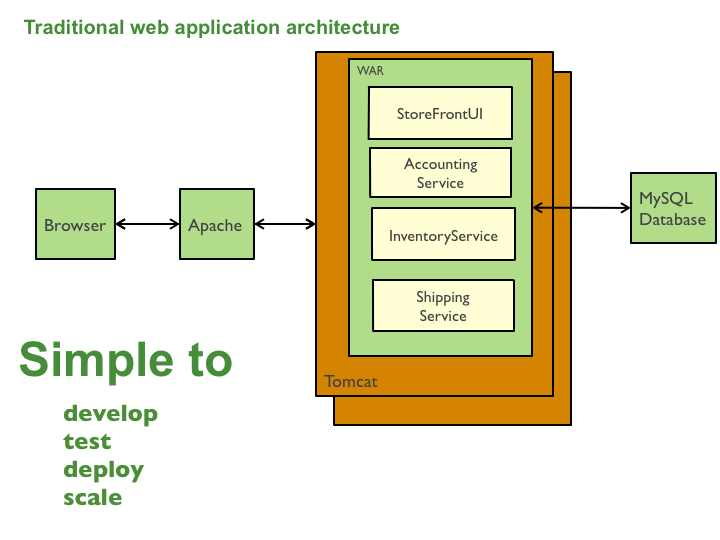
\includegraphics[width=0.9\linewidth]{images/TraditionalWebArchitecture}
		\caption{Traditionelle monolithische Webanwendungs-Architektur}
		\label{fig:TraditionalWebArchitecture}
	\end{figure}

	\cite*{Richardson.2014} sieht jedoch auch eine Reihe von Nachteilen dieser Architektur, die mit zunehmender Größe der Anwendung und wachsender Teamgröße immer signifikanter werden.
	
	\begin{itemize}
	\item Die große monolithische Codebasis kann neue Entwickler schnell einschüchtern. Änderungen und Verständnis können schwierig sein und die Entwicklung verlangsamen. Durch fehlende Modulgrenzen geht im laufe der Zeit die Modularität verloren.
	\item Mit wachsender Größe er Codebasis werden die Integrierte Entwicklungsumgeben (IDE) langsamer und bremsen die Produktivität
	\item Anwendungsstart wird zunehmend länger und hat einen großen Effekt auf die Produktivität der Entwickler und die Auslieferung. Wartezeit ist verschwendete Zeit.
	\item \textbf{Continuous deployment is difficult }
	\item Das Skalieren der Anwendung kann schwierig werden, da es nur in eine Dimension skalieren kann. Mit wachsenden Transaktionen kann das System durch zusätzlich Instanzen skaliert werden. Hingegen kann bei einem wachsenden Datenvolumen diese Architektur nicht gut skalieren. Jede Instanz greift auf alle Daten zurück und führt zu wenig effektivem Caching, höherem Speicherverbrauch sowie zusätzlichem I/O traffic. Außerdem können unterschiedliche Anwendungsbereiche verschiedene Anforderungen z.B. CPU haben. Das skalieren von einzelnen Komponenten ist jedoch unmöglich.
	\item Die monolithische Architektur hat Grenzen wie die Entwicklung skalieren kann. Bei einer entsprechenden Anwendungsgröße werden Teams gebildet, die für spezielle Bereiche verantwortlich sind z.B. UI Team, Buchhaltungs Team etc.
	Die enge Verzahnung der einzelnen Bereiche erschwert jedoch die unabhängige Arbeit.
	\item Mit dem Beginn der Entwicklung muss sich auf eine Technologie und ggf. eine Version festgelegt werden, die es sehr schwer macht neue Technologien zu adaptieren. Eine inkrementelle Umstellung gestaltet sich als schwierig, wobei eine vollständige Ersetzung der aktuellen Technologie sehr kostenintensiv ist und das Problem im Kern nicht behebt, da sich wieder auf eine neue Technologie für das Ganze festgelegt werden muss.
	\end{itemize}
	
	\subsection{Client/Server-Architekturmodell}
	Im Gegensatz zur monolitischen Architektur handelt es sich beim Client/Server Modell um ein verteiltes System.
	Das Client/Server-Architekturmodel ist ein Systemmodell, das aus einer Anzahl von zugehörigen Diensten und Servern besteht, sowie aus Clients, die diese Dienste nutzen und auf sie zugreifen. Das einfachste Modell ist dabei das zweischichtige Client/Server Modell, die zusammen ein komplettes System bilden mit unterschiedlichen Zuständigkeiten. \\
	Dabei lassen sich drei logische Hauptbestandteile unterschieden.
	
	\begin{figure}[h]
		\centering
		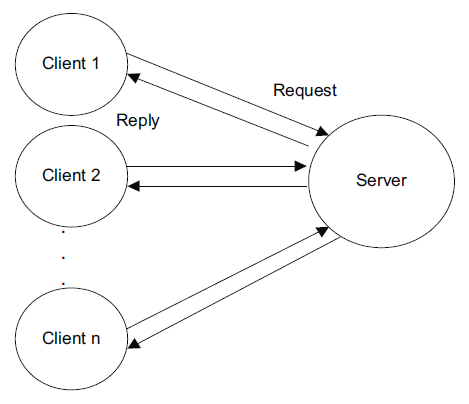
\includegraphics[width=0.5\linewidth]{images/Clients-und-Server}
		\caption{Client Server Model}
		\label{fig:client-server}
	\end{figure}
	
	\paragraph{Server}
	Der Server ist die zentrale Einheit der Architektur. Sie stellt Services und Daten anderen Einheiten zur Verfügung. Der Server muss nicht zwingend wissen, welche und wie viele Einheiten die von ihm zur Verfügung gestellten Dienste und Daten nutzen.
	
	\paragraph{Client}
	Clients können in beliebig großer Anzahl existieren. Sie nehmen die Daten oder Services, die vom Server bereitgestellt werden in Anspruch. Um mit den Diensten interagieren zu können, muss ein Client von der Existenz und dessen Adresse wissen. Der Client sendet eine Anfrage an den Server und bekommt ein Resultat zurück geliefert. \citet*[S. 302]{Sommerville.2007} unterscheidet folgende zwei Client-Modelle:
	\\
	\\
	\textbf{Thin-Client-Modell}\\
	Bei diesem Modell werden die gesamten Anwendungsprozesse und Datenhaltung auf dem Server erledigt. Der Client ist nur für die Darstellung verantwortlich. Daraus ergibt sich der Vorteil, dass sehr wenig Ressourcen für den Client benötigt werden und dieser sich auch auf kleinen Systemen (z.B. Terminals) implementieren lässt. Der Nachteil dieses Modelles liegt jedoch darin, dass so sämtliche Arbeit Serverseitig geleistet werden muss. Gerade bei Anwendungen mit großer Client Anzahl oder rechenintensiven Operationen kann so der Server schnell zur kritischen Komponente werden und das System vor Skalierungsprobleme stellen. Zusätzlich führt der Thin-Client zu einer erhöhten Netzwerkbelastung, da alle Daten vom Server zum Client transportiert werden müssen.
	\\
	\\
\textbf{Fat-Client-Modell}\\
	Dieses Modell verlagert die Anwendungslogik vollständig oder in großen Teilen vom Server direkt in den Client. Dadurch kann der Server deutlich entlastet werden und die Rechenleistung des Client Rechners zusätzlich genutzt werden. Dies kann sich in speziellen Situationen allerdings auch als Nachteile erweisen, wenn die Client Computer die notwendige Rechenleistung nicht selbstständig bereitstellen könne. Der Server fungiert dabei nur noch als Daten Service und die Netzwerklast wird reduziert. Die Verlagerung der Anwendungslogik auf den Client bringt aber auch Nachteile mit sich. Müssen hier Änderungen vorgenommen werden, so müssen alle Clients auf die neue Version aktualisiert werden, was zu einem komplexen Systemmanagement führen kann. Der Aufwand dafür steigt mit zunehmender Zahl der Clients.
	
	\paragraph{Netzwerk (optional)}
	In der Literatur wird das Netzwerk häufig noch als dritter Bestandteil aufgeführt, der jedoch nicht zwingend notwendig ist da prinzipiell Server und Client auf einem Computer ausgeführt werden können und so kein Netzwerk zur Kommunikation benötigen. Da dieses Modell aber in der Praxis nahezu ausschließlich als verteiltes System angewendet wird, ist in diesen Fällen das Netzwerk grundlegende Kommunikationsgrundlage.
	
	Generell hat das zweischichtige Client/Server Modell das Problem, dass die drei logischen Schichten auf zwei unterschiedlichen Computersystemen abgebildet werden müssen. \\
	
	\begin{figure}[h]
		\centering
		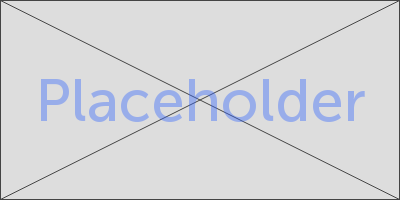
\includegraphics[width=0.5\linewidth]{images/placeholder}
		\caption{Logische drei Schichten}
		\label{fig:log3schichten}
	\end{figure}
	
	Als Weiterentwicklung hat sich dafür die dreischichtige System-Architektur Entwickelt. Sie stellt für jede logische Schicht ein separates Computersystem zur Verfügung. Die Vorteile liegen dabei in der besseren Skalierbarkeit, da jedes System individuell skaliert werden kann, geringere Netzwerklast im Vergleich zum Thin-Client-Modell und Anwendungsprozesse sind zentralisiert und lassen sich dort leichter anpassen und aktualisieren.
	

	\begin{figure}[h]
		\centering
		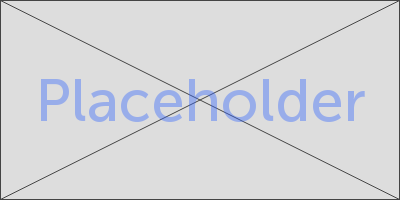
\includegraphics[width=0.5\linewidth]{images/placeholder}
		\caption{Dreischichtige Architektur}
		\label{fig:3-tier-architecture}
	\end{figure}


	\citet*{Sommerville.2007} gibt in seinem Buch Software Engineering Beispiele, wann die Anwendung der jeweiligen Architektur sinnvoll ist.
	
	\begin{table}[h]
	\begin{tabular}{|p{3.5cm}|p{12.5cm}|}
		\hline 
		\textbf{Architektur} & \textbf{Anwendung} \\ 
		\hline 
		Zweischichtige C/S-Architektur mit Thin-Clients & Anwendungen mit Legacy-Systemen, bei denen die Trennung von Anwendungsprozessen und Datenmanagement nicht praktikabel ist. Rechenintensive Anwendungen wie zum Beispiel Compiler mit geringem oder keinem Datenmanagement. Datenintensive Anwendungen (Browser oder Abfragesysteme) mit wenig oder keinen Anwendungsprozessen \\
		\hline 
		Zweischichtige C/S-Architektur mit Fat-Clients & Anwendungen, bei denen die Prozesse durch Standardanwendungen (z.b. Microsoft Excel) auf dem Client verarbeitet werden. Anwendungen mit rechenintensiver Datenverarbeitung (z.B. Datenvisualisierung). Anwendungen mit relativ stabiler Endbenutzerfunktionalität, die in einer Umgebung mit gut strukturiertem Systemmanagement angeordnet sind \\ 
		\hline 
		Drei- oder mehrschichtige C/S-Architektur & Anwendungen großen Umfangs mit Hunderten oder Tausenden von Clients. Anwendungen, bei denen sowohl die Daten als auch die Anwendung selbst ständigen Veränderungen unterliegen. Anwendungen, bei denen Daten aus vielfältigen Quellen verarbeitet werden \\ 
		\hline 
	\end{tabular} 
			\caption{Verwendungsbeispiele von mehrschichtigen Architekturen \cite{Sommerville.2007}}
	\end{table}
	
	
	\subsection{Dienstbasiert}
	Neben den beiden bereits genannten Architekturen hat sich eine weitere Form verbreitet. Der Schwerpunkt wird dabei auf eigenständige Dienste als primäre Komponente gelegt, auf die über eine Art von Remote-Protokoll zugegriffen werden kann. Die Art des Protokolls ist dabei nicht festgelegt oder auf eines beschränkt wie z.B. Representational State Transfer (REST), Simple Object Access Protocol (SOAP), Advanced Message Queuing Protokol (AMQP) oder andere.
	Dienstbasierten Architekturen werden signifikante Vorteile im Bezug auf Skalierbarkeit, Entkopplung, Kontrolle über die Entwicklung, Testing und Deployment zugeschrieben. Verteilte Systeme tendieren zudem dazu weniger abhängig und besser modular aufgebaut zu sein. Im Zusammenhang mit dienstabasierten Architekturen bedeutet das, das jeder Dienst eine in sich geschlossen Einheit bildet, die von einem Team selbst designed, entwickelt, getestet und ausgeliefert wird.  Abhängigkeiten zu anderen Komponenten sollten dabei nicht, oder nur minimal bestehen. \\
	Diese Vorteile bringen jedoch auch einige Nachteile mit sich, so zählen erhöhte Komplexität und höhere initiale Kosten zu den meist genannten Argumenten.
	
	\paragraph{Representalional State Transfer (REST)}
		REST wurde erstmals 2000 von Roy Thomas Fielding in seiner Dissertation beschrieben. Im Gegensatz zu bekannten Protokollen wie Simple Object Access Protokol (SOAP) oder XML-RPC handelt es sich bei REST um einen Architekturstil, wie Anwendungen basierend auf dem HTTP Protokoll miteinander kommunizieren können. Unterstützt eine Anwendung die REST-Stil, so bezeichnet man sie als RESTful.
		\cite[vgl.][]{Melzer.2010} \\
		REST basiert auf einem Konzept von Ressourcen, über die der Service Kenntnis hat. Der Server erstellt dabei verschiedene Darstellungen, wobei diese entkoppelt ist von der internen Speicherung.
		HTTP und HTTPS sind die primär benutzten Protokolle bei der Verwendung von REST. HTTP Caching Proxies, Load-Balancers und Monitoring Tools besitzen einen tiefe Unterstützung für HTTP von Haus aus, die in der Entwicklung hilfreiche Dienste leisten.
		Den HTTP Verben GET, POST, PUT und DELETE lösen in RESTful Anwendungen spezielle Aktionen aus (siehe Tabelle~\ref{tbl:RestOperationen}).
		\\
		
		\begin{table}[h]
		
		\begin{tabular}{|p{3.5cm}|p{12.5cm}|}
		\hline 
		\textbf{HTTP Verb} & \textbf{REST Aktion} \\ 
		\hline 
		GET & Abfragen einer Ressource ohne Änderungen vorzunehmen \\ 
		\hline 
		POST & Erstellt eine neue Ressource. Der Link zur neuen Ressource wird zurück gegeben \\ 
		\hline 
		PUT & Eine Ressource wird angelegt. Wenn die Ressource bereits existiert, wird sie geändert. \\ 
		\hline 
		PATCH & Ein Teil der Ressource wird geändert \\ 
		\hline 
		DELETE & Löscht eine Ressource \\ 
		\hline 
		\end{tabular} 
		\caption{Rest Operationen}
		\label{tbl:RestOperationen}
		\end{table}
		
		Der große Vorteil und der Grund für die schnelle Verbreitung von REST Architekturen liegt in der Einfachheit. Methoden für die Nutzung des HTTP Protokoll sind in allen modernen Programmiersprachen enthalten und können einfach genutzt werden. Das Ressourcen Konzept ist leicht anwendbar und bietet umfangreiche Möglichkeiten der eigenen Anpassung.
		
		Die Bandbreite der Möglichkeiten, die mit der REST Architektur umgesetzt werden können zeigt Leonard Richardson in seinem \textacutedbl Richardson Maturity Model\textgravedbl  indem er vier REST Level beschreibt.
	
		\begin{figure}[h]
			\centering
			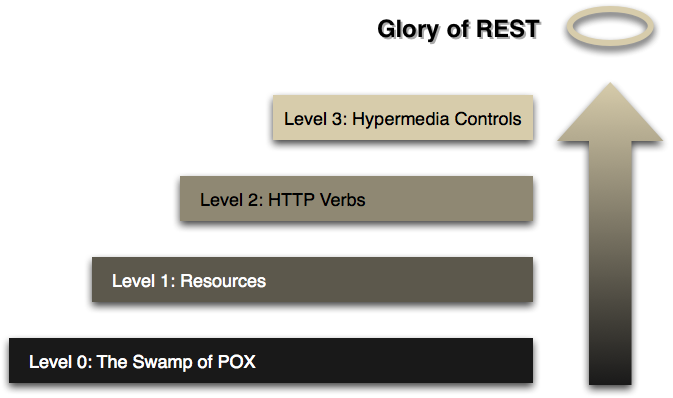
\includegraphics[width=0.7\linewidth]{images/Richardson_Maturity_Model}
			\caption{Richardson Maturity Model}
			\label{fig:Richardson_Maturity_Model}
		\end{figure}
		
		\cite[vgl.][]{Fowler.2010}


\section{SaaS spezifische Besonderheiten}
\subsection{Multi-Tenant Application (MTA)}
Bevor die MTA im Detail erklärt werden kann, ist es wichtig ein gemeinsames Verständnis von Tenant (dt. Mieter) und Multi-Tenancy (dt. Mehrfach Mieter) im Kontext von Software-Anwendungen zu schaffen. \cite*[vgl. ][S.2]{Krebs.2012}
\\

\textbf{Tenant:} Bezeichnet eine Gruppe von Benutzern, die die gleiche Sicht auf eine Software teilen. Dies bezieht sich auf die Punkte wie zugreifbare Daten, Konfiguration, User Management und Funktionalität. Ein Tenant ist häufig eine (Teil-)Organisation wie zum Beispiel eine Hochschulsporteinrichtung. \\ 

\textbf{Multi-Tenancy:} Beschreibt ein Modell bei dem eine Anwendungsinstanz von mehreren Tenants genutzt wird aber jeder einen eingeschränkten, isolierten Zugriff erhält. Dabei werden Performance und Datenschutz Kriterien je Tenant behandelt. \\ 

\textbf{Multi-Tenant Application:} Teilt eine Anwendungsinstanz unter mehreren Tenants, um zusätzliche Kosten zu reduzieren. 
\\ 

Die primäre Herausforderung in MTA liegt daher in der sauberen Trennung von Abläufen und Daten zwischen den einzelnen Tenants. \cite{Chong.2006} zeigen in ihrem Artikel drei unterschiedliche Möglichkeiten, wie Multi-Tenant Daten verwaltet werden können.

\paragraph{Separierte Datenbanken}
In diesem Ansatz werden die Daten für jeden Tenant in einer eigenen Datenbank gespeichert (vgl. Abbildung~\ref{fig:separierteDatenbanken}). Die Hardware Ressourcen und der Anwendungscode werden dabei geteilt. Innerhalb des Datenbank Management Systems (DBMS) bekommt jeder Tenant jedoch eine eigene Datenbank und auf Datenbankzugriffsebene wird eine Trennung zu anderen Nutzern hergestellt. Dadurch können mit dieser Methode Sicherheits- und Datenschutzaspekte am besten bedient werden. Dieser Ansatz macht es einfach das Datenmodell individuell zu erweitern und Daten aus einem Backup wiederherzustellen. Anderseits führt es zu höheren Wartungskosten, da mehrere Datenbanken verwaltet werden müssen und das Backup Prozedere komplizierter wird. Zusätzlich ist in einigen DBMS die Anzahl der Datenbanken beschränkt, sodass bei einer hohen Tenant Anzahl zusätzliche DBMS benötigt werden.

\begin{figure}[h]
	\centering
	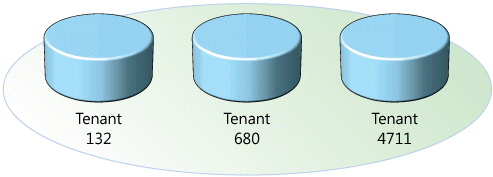
\includegraphics[width=0.7\linewidth]{images/separierte_datenbanken}
	\caption{Separierte Datenbanken}
	\label{fig:separierteDatenbanken}
\end{figure}
vgl.	
\\
\\
\paragraph{Geteilte Datenbank, separiertes Schema}
Ein alternativer Ansatz ist es, alle Tenant Daten innerhalb einer Datenbank zu speichern, wobei jeder ein eigenes Schema und Set von Tabellen mit entsprechenden Zugriffsrechten bekommt.
Die Implementierung ist relativ einfach und erreicht ein gemäßigtes Maß an logischer Isolation (vgl. Abbildung~\ref{fig:geteilteDatenbank}). Im Gegensatz zum Ansatz mit separierten Datenbanken lassen sich so jedoch deutlich mehr Tenants unterstützen. Das Wiederherstellen von Tenant spezifischen Daten aus einem Backup gestaltet sich in diesem Ansatz deutlich schwieriger. Da ein Datenbank Backup nicht einfach zurück gespielt werden kann, müssen zuerst alle Daten aller Tenants aus einem Backup in einen Temporären Server zurück gespielt werden, um sie anschließend von dort zurück in das Produktivsystem spielen zu können. Diese Vorgehensweise führt zu einem erheblichen Mehraufwand im Falle von Datenverlust.

\begin{figure}[h]
	\centering
	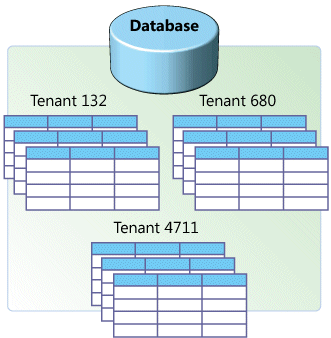
\includegraphics[width=0.5\linewidth]{images/geteilte_datenbanken-separiertes_schema}
	\caption{Geteilte Datenbank und separierte Schemata}
	\label{fig:geteilteDatenbank}
\end{figure}
vgl.
\\
\\
\paragraph{Geteilte Datenbank, geteiltes Schema} 
Dieser Ansatz basiert auf einer Datenbank und einem Set von Tabellen. Die Trennung der Daten erfolgt über das Mitführen einer Tenant-ID in jedem Datensatz wie in Abbildung~\ref{fig:geteilteDatenbankundSchema} zu sehen. Diese Lösungsstrategie erlaubt die Versorgung einer großen Tenant-Anzahl per Datenbank und erfordert daher die geringsten Hardware und Backup Kosten. Gleichzeitig erfordert es auch den höchsten Aufwand die Trennung von Tenant Daten anwendungsseitig sicherzustellen, um alle Sicherheits- und Datenschutzbedingungen zu erfüllen. Die Probleme beim Wiederherstellen von Backups verhalten sich wie beim Ansatz mit separiertem Schema. 
\begin{figure}[h]
	\centering
	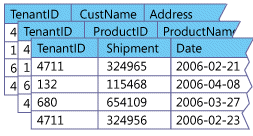
\includegraphics[width=0.5\linewidth]{images/geteilte_datenbank-geteiltes_schema}
	\caption{Geteilte Datenbank und Schema}
	\label{fig:geteilteDatenbankundSchema}
\end{figure}
vgl.
\\
\\
adfkadf 
\subsection{Security}
